% Economic Bandits — Chapter 6

\subsection{Introduction}
\label{sec:bandits_intro}

Multi-armed bandit (MAB) problems represent a class of stateless reinforcement learning tasks where an agent repeatedly selects among different actions (arms) to maximize cumulative reward. A $K$-armed bandit is a degenerate MDP with a single state: $|\mathcal{S}| = 1$, action set $\mathcal{A} = \{1, \ldots, K\}$ (arms), and reward $r_t \sim \nu_{a_t}$ drawn from arm $a_t$'s distribution with mean $\mu_{a_t} = \mathbb{E}[r_t \mid a_t]$. There is no state transition or discounting. Unlike full reinforcement learning, which is typically run in simulation, bandits are often deployed in real time, making sample efficiency and optimal exploration critical.

The central concept for evaluating bandit algorithms is \emph{regret}, which measures the difference between the expected reward under an optimal strategy and the expected reward obtained by the algorithm:
\begin{equation}
R(T) = T \cdot \max_{i} \mu_i - \mathbb{E}\left[\sum_{t=1}^{T} r_t\right]
\label{eq:regret}
\end{equation}
where $\mu_i$ is the expected reward of arm $i$ and $r_t$ is the observed reward at time $t$. Lower regret indicates better performance. For general $K$-armed bandits, the minimax optimal regret scales as $\Theta(\sqrt{KT})$; no algorithm can do better against a worst-case instance.

The thesis of this chapter is that economic structure can dramatically improve this baseline. When the reward function satisfies structural assumptions motivated by economic theory, such as monotone demand curves, budget constraints, or strategic equilibrium conditions, regret bounds improve from the agnostic $O(\sqrt{T})$ rate to $O(\log T)$, representing an exponential gain in learning efficiency. This gain is not merely theoretical: field experiments in pricing and advertising consistently show that structure-aware algorithms outperform agnostic ones by large margins, often achieving the same performance with an order of magnitude fewer samples.

The sections that follow develop this theme across several domains. Section~\ref{sec:classical_bandits} reviews the classical bandit algorithms that serve as baselines. Sections~\ref{sec:dynamic_pricing} through~\ref{sec:budget_constraints} examine three core economic applications: dynamic pricing, auction design, and budget-constrained allocation. Section~\ref{sec:strategic_interactions} considers multi-agent settings where strategic behavior introduces additional structure. Section~\ref{sec:bandits_discussion} synthesizes the findings and discusses open problems.

We adopt common notation throughout the chapter. There are $K$ arms, a horizon of $T$ rounds, and arm $i$ has mean reward $\mu_i$ with optimal mean $\mu^* = \max_i \mu_i$. The suboptimality gap for arm $i$ is $\Delta_i = \mu^* - \mu_i$, and $\Delta_{\min} = \min_{i:\mu_i < \mu^*} \Delta_i$ denotes the minimum gap. Let $N_i(t)$ be the number of times arm $i$ has been pulled through round $t$ and $\hat{\mu}_i(t) = N_i(t)^{-1} \sum_{s \leq t} r_s \mathbb{1}\{a_s = i\}$ the sample mean reward. Cumulative regret $R(T)$ is defined in~\eqref{eq:regret}. In the pricing sections, $\mathcal{P} = \{p_1, \ldots, p_K\}$ is the price set, $\theta(p)$ the demand (purchase probability) at price $p$, and $p\theta(p)$ the expected revenue. In the auction sections, $r$ is the reserve price, $\mathbf{b} = (b_1, \ldots, b_N)$ the bid profile, and $v_i$ bidder $i$'s valuation. In the budget-constrained sections, $B$ is the total budget, $C_t(a)$ the cost and $X_t(a)$ the reward of action $a$ at time $t$, and $\lambda_t$ the dual variable for the budget constraint.

\subsection{Classical Bandit Algorithms}
\label{sec:classical_bandits}

Before examining how economic structure improves bandit performance, we establish the baseline: what can be achieved without structural assumptions? Three foundational algorithms define the landscape.

The simplest exploration strategy is $\varepsilon$-greedy: at each round, the agent plays the arm with the highest estimated mean reward with probability $1 - \varepsilon$, and a uniformly random arm with probability $\varepsilon$. With a fixed exploration rate $\varepsilon > 0$, regret grows linearly in $T$ because the agent never stops exploring suboptimal arms. With a decaying schedule $\varepsilon_t = \min\{1, cK/t\}$ for an appropriate constant $c$, regret can be brought to $O(T^{2/3})$, but this remains far from optimal.

\citet{LaiRobbins1985} established the fundamental lower bound on regret for any consistent policy.\footnote{A policy is \emph{consistent} if $\mathbb{E}[N_i(T)] = o(T^a)$ for every suboptimal arm $i$ and every $a > 0$, where $N_i(T)$ counts the number of times arm $i$ is played.} For a $K$-armed bandit with reward distributions from a one-parameter exponential family, any consistent policy satisfies
\begin{equation}
\liminf_{T \to \infty} \frac{R(T)}{\log T} \geq \sum_{i : \mu_i < \mu^*} \frac{\Delta_i}{\mathrm{KL}(\nu_i, \nu^*)}
\label{eq:lai_robbins}
\end{equation}
where $\Delta_i = \mu^* - \mu_i$ is the suboptimality gap for arm $i$, $\mu^* = \max_j \mu_j$ is the optimal mean, and $\mathrm{KL}(\nu_i, \nu^*)$ is the Kullback-Leibler divergence between the reward distribution of arm $i$ and the optimal arm. This instance-dependent bound shows that $\Omega(\log T)$ regret is unavoidable; the rate at which each suboptimal arm must be explored is governed by how statistically distinguishable it is from the best arm.

\citet{auer2002} introduced the UCB1 algorithm, which achieves the Lai-Robbins rate up to constant factors without requiring knowledge of the reward distributions. UCB1 selects at each round the arm maximizing an upper confidence index:
\begin{equation}
a_t = \arg\max_{i \in \{1, \ldots, K\}} \left[\hat{\mu}_i(t) + \sqrt{\frac{2 \ln t}{N_i(t)}}\right]
\label{eq:ucb1}
\end{equation}
where $\hat{\mu}_i(t)$ is the sample mean reward of arm $i$ and $N_i(t)$ is the number of times it has been played through round $t$. The exploration bonus $\sqrt{2 \ln t / N_i(t)}$ shrinks as an arm is played more often, automatically balancing exploration and exploitation. The finite-time regret of UCB1 satisfies
\begin{equation}
R(T) \leq \sum_{i : \mu_i < \mu^*} \left(\frac{8 \ln T}{\Delta_i}\right) + \left(1 + \frac{\pi^2}{3}\right) \sum_{i=1}^{K} \Delta_i
\label{eq:ucb1_regret}
\end{equation}
which is $O(K \log T / \Delta_{\min})$ for instance-dependent regret and $O(\sqrt{KT \log T})$ in the worst case, nearly matching the minimax lower bound $\Omega(\sqrt{KT})$.

Thompson Sampling, introduced by \citet{Thompson1933}, takes a Bayesian approach. The agent maintains a posterior distribution $\pi_t(\mu_i)$ over each arm's mean reward and, at each round, samples $\tilde{\mu}_i \sim \pi_t(\mu_i)$ for every arm, then plays $a_t = \arg\max_i \tilde{\mu}_i$. For Bernoulli rewards with a Beta prior, the posterior update is conjugate: if the prior is $\text{Beta}(\alpha_i, \beta_i)$, a success increments $\alpha_i$ and a failure increments $\beta_i$. Despite its simplicity, Thompson Sampling achieves the Lai-Robbins lower bound asymptotically \citep{auer2002} and often outperforms UCB1 empirically due to more adaptive exploration. The algorithm is particularly natural in economic settings where Bayesian updating reflects a decision-maker's belief revision.

\subsubsection{Simulation Study: Classical Algorithms on a Gaussian Bandit}
\label{sec:sim_fundamentals}

We conduct a Monte Carlo experiment to compare the finite-time regret of the three classical algorithms and to verify that the empirical regret trajectories track the theoretical bounds derived above.

The environment is a $K = 10$ armed bandit with Gaussian rewards $r_t \mid a_t = i \sim \mathcal{N}(\mu_i, 1)$. The arm means are fixed at $\mu = (0.1, 0.3, 0.5, 0.7, 0.9, 1.1, 1.3, 1.5, 1.7, 2.0)$, so the optimal arm is $i^* = 10$ with $\mu^* = 2.0$ and the minimum suboptimality gap is $\Delta_{\min} = 0.3$. The horizon is $T = 10{,}000$. For $\varepsilon$-greedy we use a decaying schedule $\varepsilon_t = \min\{1, 5K/(t+1)\}$. UCB1 follows~\eqref{eq:ucb1} with initialization by playing each arm once. Thompson Sampling maintains a conjugate Gaussian posterior $\mathcal{N}(\hat{\mu}_i, 1/N_i)$ per arm with a diffuse prior $\mathcal{N}(0, 100)$. All three algorithms observe the same pre-generated reward matrix in each seed to ensure a controlled comparison. The experiment is replicated over 30 independent seeds.

Two theoretical reference curves are overlaid on the regret plot. The Lai-Robbins instance-dependent lower bound~\eqref{eq:lai_robbins} is computed from the known arm parameters as $\sum_{i:\mu_i < \mu^*} \Delta_i / \mathrm{KL}(\mathcal{N}(\mu_i, 1), \mathcal{N}(\mu^*, 1)) \cdot \ln t$, where $\mathrm{KL}(\mathcal{N}(\mu_i, 1), \mathcal{N}(\mu^*, 1)) = \Delta_i^2 / 2$ for unit-variance Gaussians. The minimax reference curve is $c \sqrt{KT}$ with a fitted constant $c$.

Figure~\ref{fig:bandit_fundamentals} displays the cumulative regret trajectories. Thompson Sampling tracks closest to the Lai-Robbins lower bound, confirming its asymptotic optimality. UCB1 incurs moderately higher regret due to its deterministic, worst-case-oriented exploration bonus, but remains logarithmic. Decaying $\varepsilon$-greedy accumulates substantially more regret with higher variance across seeds, consistent with its suboptimal $O(T^{2/3})$ theoretical rate. Table~\ref{tab:bandit_fundamentals} reports the terminal regret: Thompson Sampling achieves $134.5 \pm 5.0$, UCB1 $186.8 \pm 4.8$, and $\varepsilon$-greedy $367.1 \pm 42.9$. The tenfold difference in standard error between $\varepsilon$-greedy and the other two algorithms reflects the high variance of random exploration under a decaying schedule.

\begin{figure}[htbp]
\centering
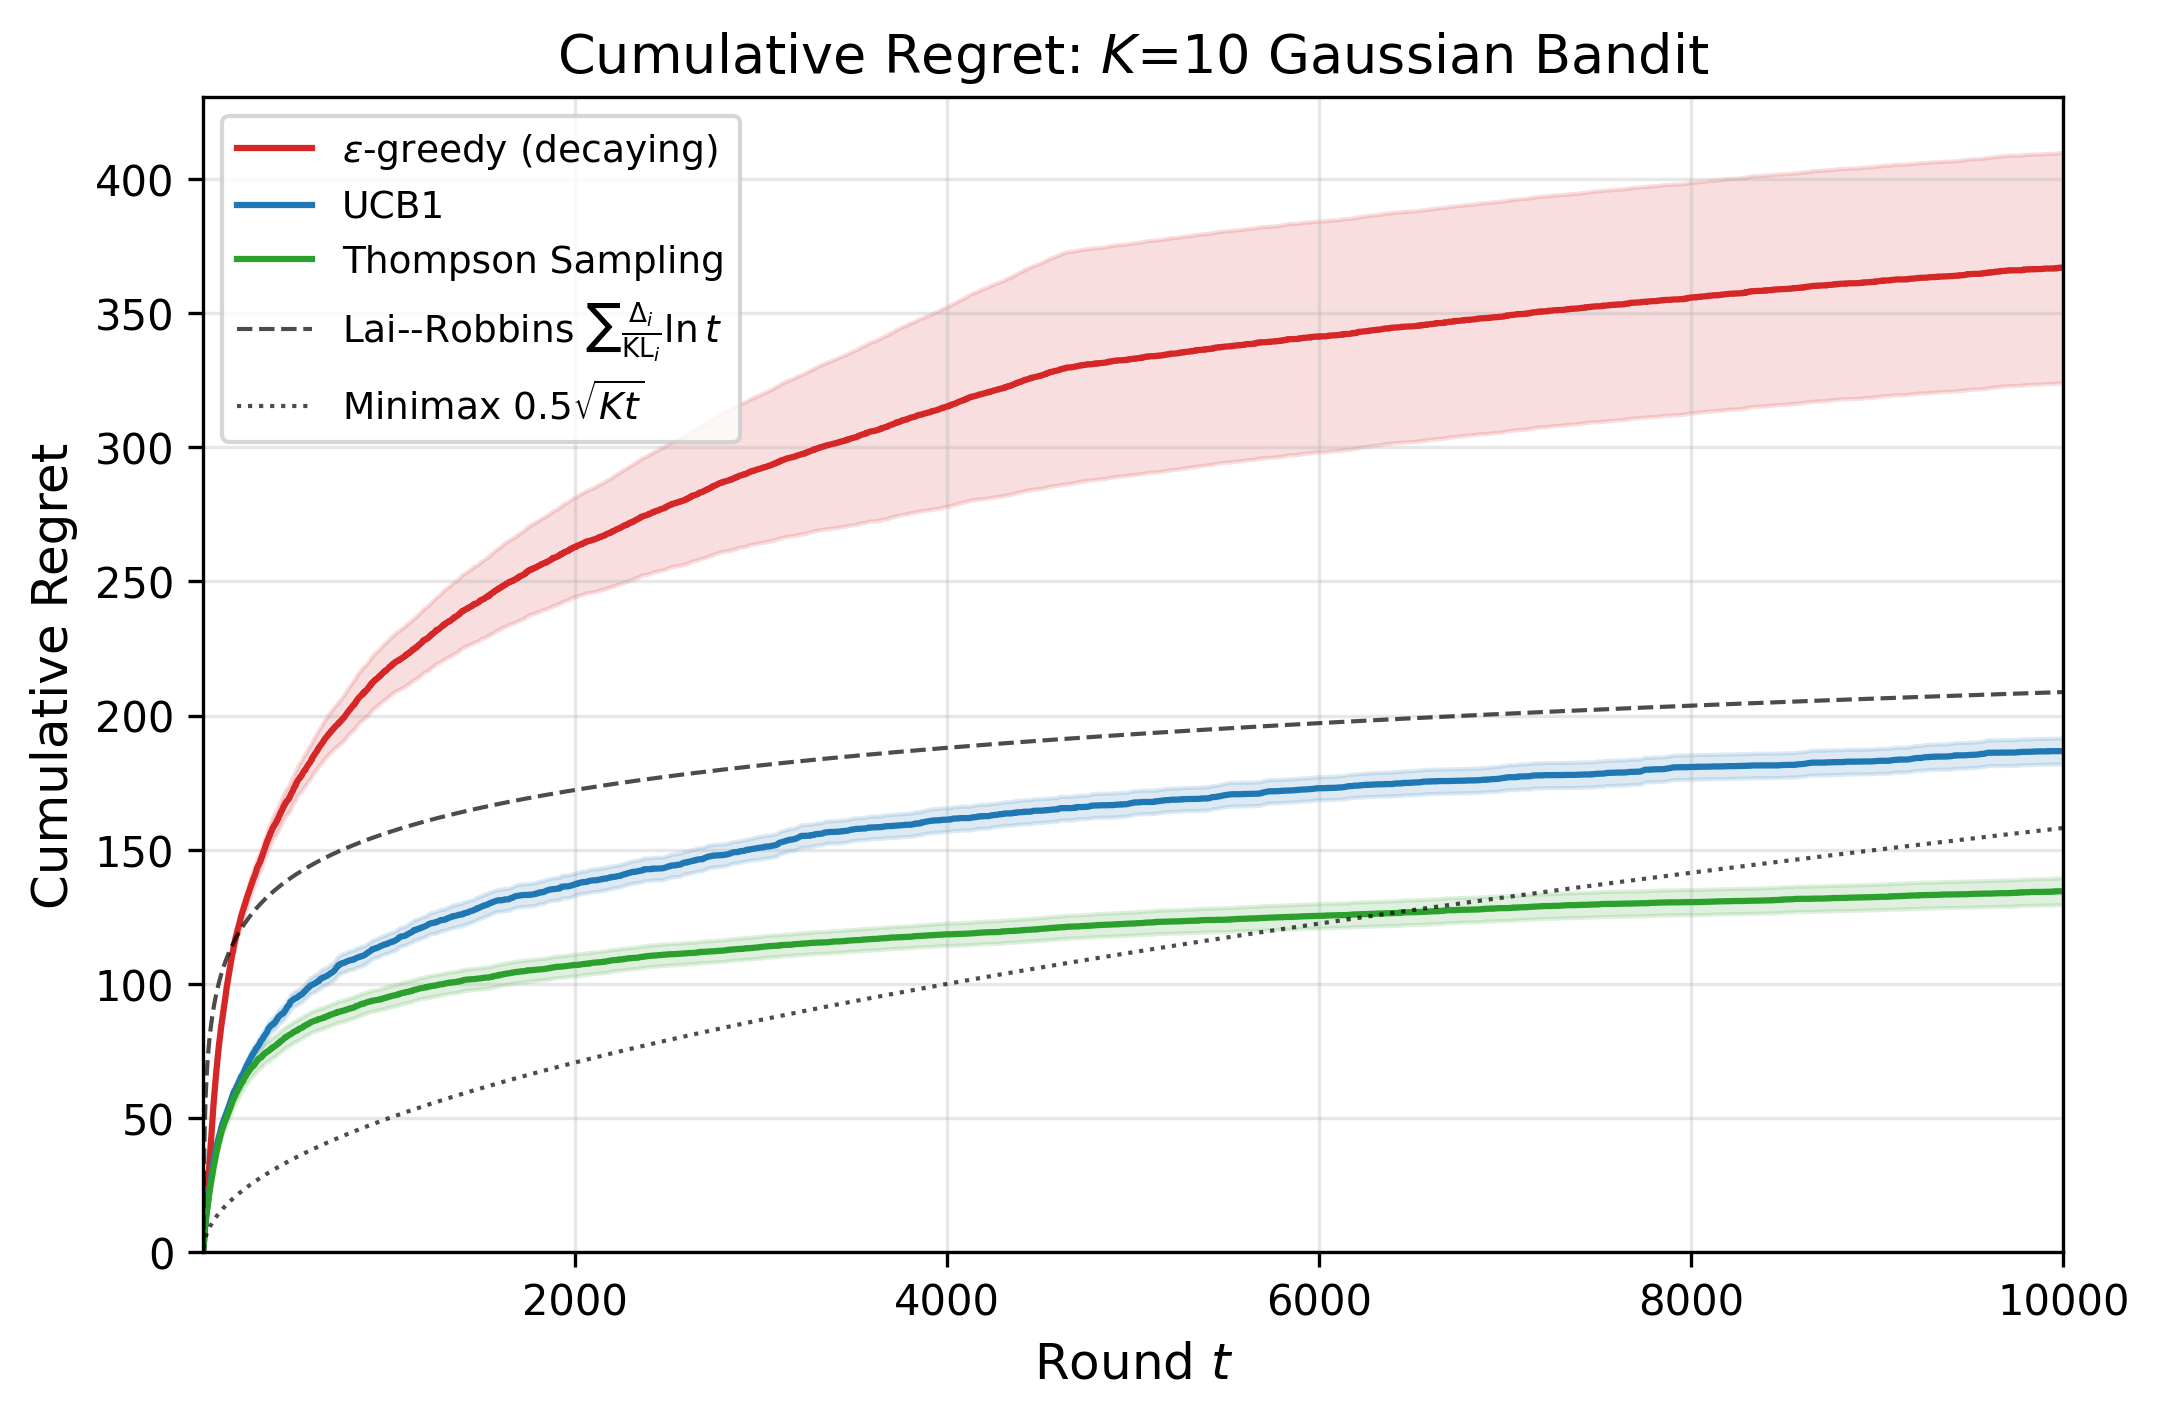
\includegraphics[width=\textwidth]{../ch06_bandits/sims/bandit_fundamentals_regret.png}
\caption{Cumulative regret of $\varepsilon$-greedy, UCB1, and Thompson Sampling on a 10-armed Gaussian bandit ($\mu^* = 2.0$, $\sigma = 1$) over $T = 10{,}000$ rounds. Solid lines are means over 30 seeds; shaded regions indicate $\pm 1$ standard error. Dashed curves show the Lai-Robbins instance-dependent lower bound (black) and the minimax $\sqrt{KT}$ reference (gray).}
\label{fig:bandit_fundamentals}
\end{figure}

\begin{table}[htbp]
\centering
\begin{tabular}{lcc}
\hline
Algorithm & Final Regret (mean $\pm$ SE) & \% Optimal Arm Pulls \\
\hline
$\varepsilon$-greedy (decaying) & 367.1 $\pm$ 42.9 & 95.4\% \\
UCB1 & 186.8 $\pm$ 4.8 & 96.8\% \\
Thompson Sampling & 134.5 $\pm$ 5.0 & 97.8\% \\
\hline
\end{tabular}
\caption{Terminal cumulative regret and fraction of plays on the optimal arm at $T = 10{,}000$ for the 10-armed Gaussian bandit. Mean $\pm$ one standard error over 30 seeds.}
\label{tab:bandit_fundamentals}
\end{table}


\subsection{Dynamic Pricing with Demand Learning}
\label{sec:dynamic_pricing}

Consider a seller facing sequential customers with unknown demand. Let $\mathcal{P} = \{p_1, \ldots, p_K\}$ be a discrete price set. At time $t$, setting price $p$ yields a sale with probability $\theta(p)$ and revenue $R_t = p \cdot \mathbb{1}\{\text{sale}\}$. Standard bandits would treat each price as independent, requiring $\Omega(K)$ exploration rounds. Microeconomic theory contributes the structural assumption that $\theta(p)$ decreases monotonically with $p$: consumers buy when their valuation exceeds the posted price. Under regularity conditions (monotone hazard rate), expected revenue $p\theta(p)$ is unimodal in $p$.

\citet{Misra2019} exploit this structure with an upper-confidence bound algorithm computing an index for each price:
\begin{equation}
I_p(t) = \hat{\mu}_p(t) + \sqrt{\frac{2\ln t}{N_p(t)}}
\end{equation}
where $\hat{\mu}_p(t)$ is the average revenue for price $p$ and $N_p(t)$ the number of times $p$ was tried. This achieves polylogarithmic regret compared to $\Omega(\sqrt{T})$ for standard bandits, representing an exponential improvement in learning efficiency. Their field experiments show 43\% higher profits compared to static pricing during a month-long deployment.

For multi-product settings, \citet{Mueller2019} consider demand:
\begin{equation}
\mathbf{q}_t = \mathbf{c}_t - \mathbf{B}_t\mathbf{p}_t + \boldsymbol{\varepsilon}_t
\end{equation}
where $\mathbf{q}_t \in \mathbb{R}^N$ is demand, $\mathbf{B}_t \in \mathbb{R}^{N \times N}$ is the price-sensitivity matrix, and $\mathbf{c}_t$ represents baseline demand. The key economic insight is imposing low-rank structure on $\mathbf{B}_t$, reflecting that cross-price elasticities are driven by a small number of latent factors. Their OPOL algorithm projects high-dimensional price vectors into a learned latent subspace, achieving regret of $O(T^{3/4}\sqrt{d})$ that scales with latent dimension $d \ll N$ rather than product count $N$. This enables efficient learning even with thousands of products.

\citet{Xu2021} demonstrate that economic structure enables logarithmic regret even in adversarial settings. For contextual pricing where valuation $v_t = \boldsymbol{\theta}^\top \mathbf{x}_t$ follows a linear model with feature vector $\mathbf{x}_t$, they achieve optimal $O(d \log T)$ regret, an exponential improvement over standard $\Omega(\sqrt{T})$ bounds for adversarial contexts.

\citet{Goyal2022} address multi-product pricing under the multinomial logit (MNL) choice model, where a consumer's utility for product $i$ is:
\begin{equation}
U_i(\mathbf{p}) = \alpha_i - \beta_i p_i + \epsilon_i
\end{equation}
and purchase probabilities follow:
\begin{equation}
\Pr(i|\mathbf{p}) = \frac{e^{U_i(\mathbf{p})}}{\sum_j e^{U_j(\mathbf{p})}}
\end{equation}
By incorporating this MNL structure into an Online Newton Step method with random price perturbations, they achieve $O(d\sqrt{T}\log T)$ regret despite adversarial context arrivals.

\subsubsection{Simulation Study: Unimodal Pricing under Logistic Demand}
\label{sec:sim_pricing}

We test whether exploiting the unimodal structure of the revenue function accelerates learning relative to agnostic exploration. The environment has $K = 20$ prices on $\{0.50, 1.00, \ldots, 10.00\}$ with logistic demand $\theta(p) = 1/(1 + \exp(1.5(p - 5)))$ and binary sale outcomes, so revenue at round $t$ is $R_t = p_{a_t} \cdot \mathbb{1}\{U_t < \theta(p_{a_t})\}$ for uniform $U_t$. The expected revenue $p\theta(p)$ is unimodal with optimum at $p^* = 4.00$ and $\mathbb{E}[\text{rev}^*] = 3.2728$. The horizon is $T = 50{,}000$.

Three algorithms are compared: decaying $\varepsilon$-greedy with $\varepsilon_t = \min\{1, 5K/(t+1)\}$; UCB1 per~\eqref{eq:ucb1}; and Unimodal UCB (UUCB), which maintains a leader arm and explores only its immediate neighbors, migrating the leader when a neighbor's sample mean exceeds the current leader's.\footnote{The UUCB design follows the leader-and-neighbor principle of \citet{CombesProutiere2014}, adapted to the discrete price grid.} All three algorithms observe the same pre-generated uniform draws in each seed, ensuring a controlled comparison. The experiment is replicated over 30 independent seeds.

Figure~\ref{fig:dynamic_pricing} displays cumulative regret trajectories (left panel) and price selection distributions (right panel). UUCB concentrates $95.9\%$ of pulls on the optimal price, achieving terminal regret of $480 \pm 30$. UCB1 reaches $848 \pm 245$, exploring more broadly across the price grid but converging to the optimum. Decaying $\varepsilon$-greedy incurs $4318 \pm 580$, with high variance reflecting the cost of undirected exploration over 20 arms. The UUCB regret curve tracks the structural $O(\log T)$ reference, while UCB1 lies between the structural and agnostic $O(\sqrt{KT})$ bounds. Table~\ref{tab:dynamic_pricing} reports the full results.

\begin{figure}[htbp]
\centering

\includegraphics[width=\textwidth]{../ch06_bandits/sims/dynamic_pricing_regret.png}
\caption{Left: cumulative regret of $\varepsilon$-greedy, UCB1, and Unimodal UCB on a logistic demand pricing problem with $K = 20$ prices over $T = 50{,}000$ rounds. Solid lines are means over 30 seeds; shaded regions indicate $\pm 1$ standard error. Dashed curves show the agnostic $O(\sqrt{Kt})$ and structural $O(\log t)$ reference rates. Right: fraction of pulls allocated to each price.}
\label{fig:dynamic_pricing}
\end{figure}

\begin{table}[htbp]
\centering
\begin{tabular}{lccc}
\hline
Algorithm & Final Regret & Fraction on Optimal & Total Revenue \\
\hline
$\varepsilon$-greedy & 4317.5 $\pm$ 580.4 & 0.512 $\pm$ 0.088 & 159224.5 $\pm$ 584.0 \\
UCB1 & 847.5 $\pm$ 245.3 & 0.890 $\pm$ 0.044 & 162637.0 $\pm$ 245.7 \\
Unimodal UCB & 480.2 $\pm$ 30.3 & 0.959 $\pm$ 0.003 & 163007.4 $\pm$ 64.2 \\
\hline
\end{tabular}

\caption{Terminal cumulative regret, fraction of rounds on the optimal price, and total revenue for dynamic pricing with $K = 20$ prices and logistic demand over $T = 50{,}000$ rounds. Mean $\pm$ one standard error over 30 seeds.}
\label{tab:dynamic_pricing}
\end{table}


\subsection{Bid Optimization in Auctions}
\label{sec:bid_optimization}

In a second-price auction with reserve $r$, given bid profile $\mathbf{b} = (b_{(1)}, b_{(2)}, \ldots)$ ordered decreasingly, revenue is:
\begin{equation}
\text{Revenue}(r,\mathbf{b}) = b_{(2)}\mathbb{1}\{b_{(2)} > r\} + r\mathbb{1}\{b_{(1)} \geq r > b_{(2)}\}
\end{equation}
Myerson's auction theory establishes that under regularity conditions, expected revenue $R(r)$ is unimodal in $r$. \citet{CesaBianchi2015} leverage this in a unimodal bandit algorithm maintaining two UCB indices bracketing the current best reserve, achieving $O(\log T)$ regret in favorable cases, a significant improvement over the $O(\sqrt{T})$ regret of standard bandits.

\citet{Akcay2022} address the partial feedback challenge where losing bids are unobserved. Their algorithm incorporates auction rules into inference: if a sale occurs at price $r$, exactly one bid exceeded $r$, informing future exploration. These auction-specific inference rules convert censored observations into side information, accelerating learning in both stationary and non-stationary environments.

\subsubsection{Simulation Study: Reserve Price Learning in Second-Price Auctions}
\label{sec:sim_auction}

We evaluate whether unimodal structure in the expected revenue curve over reserve prices translates into faster learning in an auction environment with high per-round variance. The environment has $N = 3$ bidders with i.i.d.\ valuations drawn from $\text{LogNormal}(0, 0.5)$, $K = 25$ reserve prices on $\{0.20, 0.40, \ldots, 5.00\}$, and a second-price auction mechanism. The Myerson optimal reserve is $r^* = 0.7719$, computed by solving $\phi(v) = v - (1 - F(v))/f(v) = 0$ numerically. The horizon is $T = 20{,}000$.

Two algorithms are compared against the Myerson oracle (which always sets the optimal reserve). UCB1 initializes by playing each arm once and then follows~\eqref{eq:ucb1}. Unimodal UCB uses a 5-round-per-arm warm-up phase (125 total rounds), then maintains a leader arm with neighbor-only exploration as in Section~\ref{sec:sim_pricing}. Both algorithms observe pre-generated bid matrices, and the experiment is replicated over 30 seeds.

Figure~\ref{fig:auction_reserve} shows cumulative regret (left) and the expected revenue curve overlaid with exploration distributions (right). UCB1 achieves terminal regret of $613 \pm 6$, capturing $97.1\%$ of Myerson optimal revenue. UUCB performs worse: terminal regret $1093 \pm 421$ ($94.9\%$ of Myerson), with an order-of-magnitude larger standard error. This is an honest negative result. The expected revenue surface is flat near the peak: the four lowest reserve arms ($r \in \{0.20, 0.40, 0.60, 0.80\}$) lie within $0.007$ of each other in expected revenue. Combined with the high variance of binary auction outcomes (revenue is either zero or the clearing price), the UUCB leader migration mechanism fails to reliably distinguish neighbors, causing the leader to drift across the flat region rather than lock onto the optimum. UCB1's broader exploration compensates by sampling the entire grid, ultimately concentrating on the best arm more reliably. Table~\ref{tab:auction_reserve} reports the full results.

\begin{figure}[htbp]
\centering
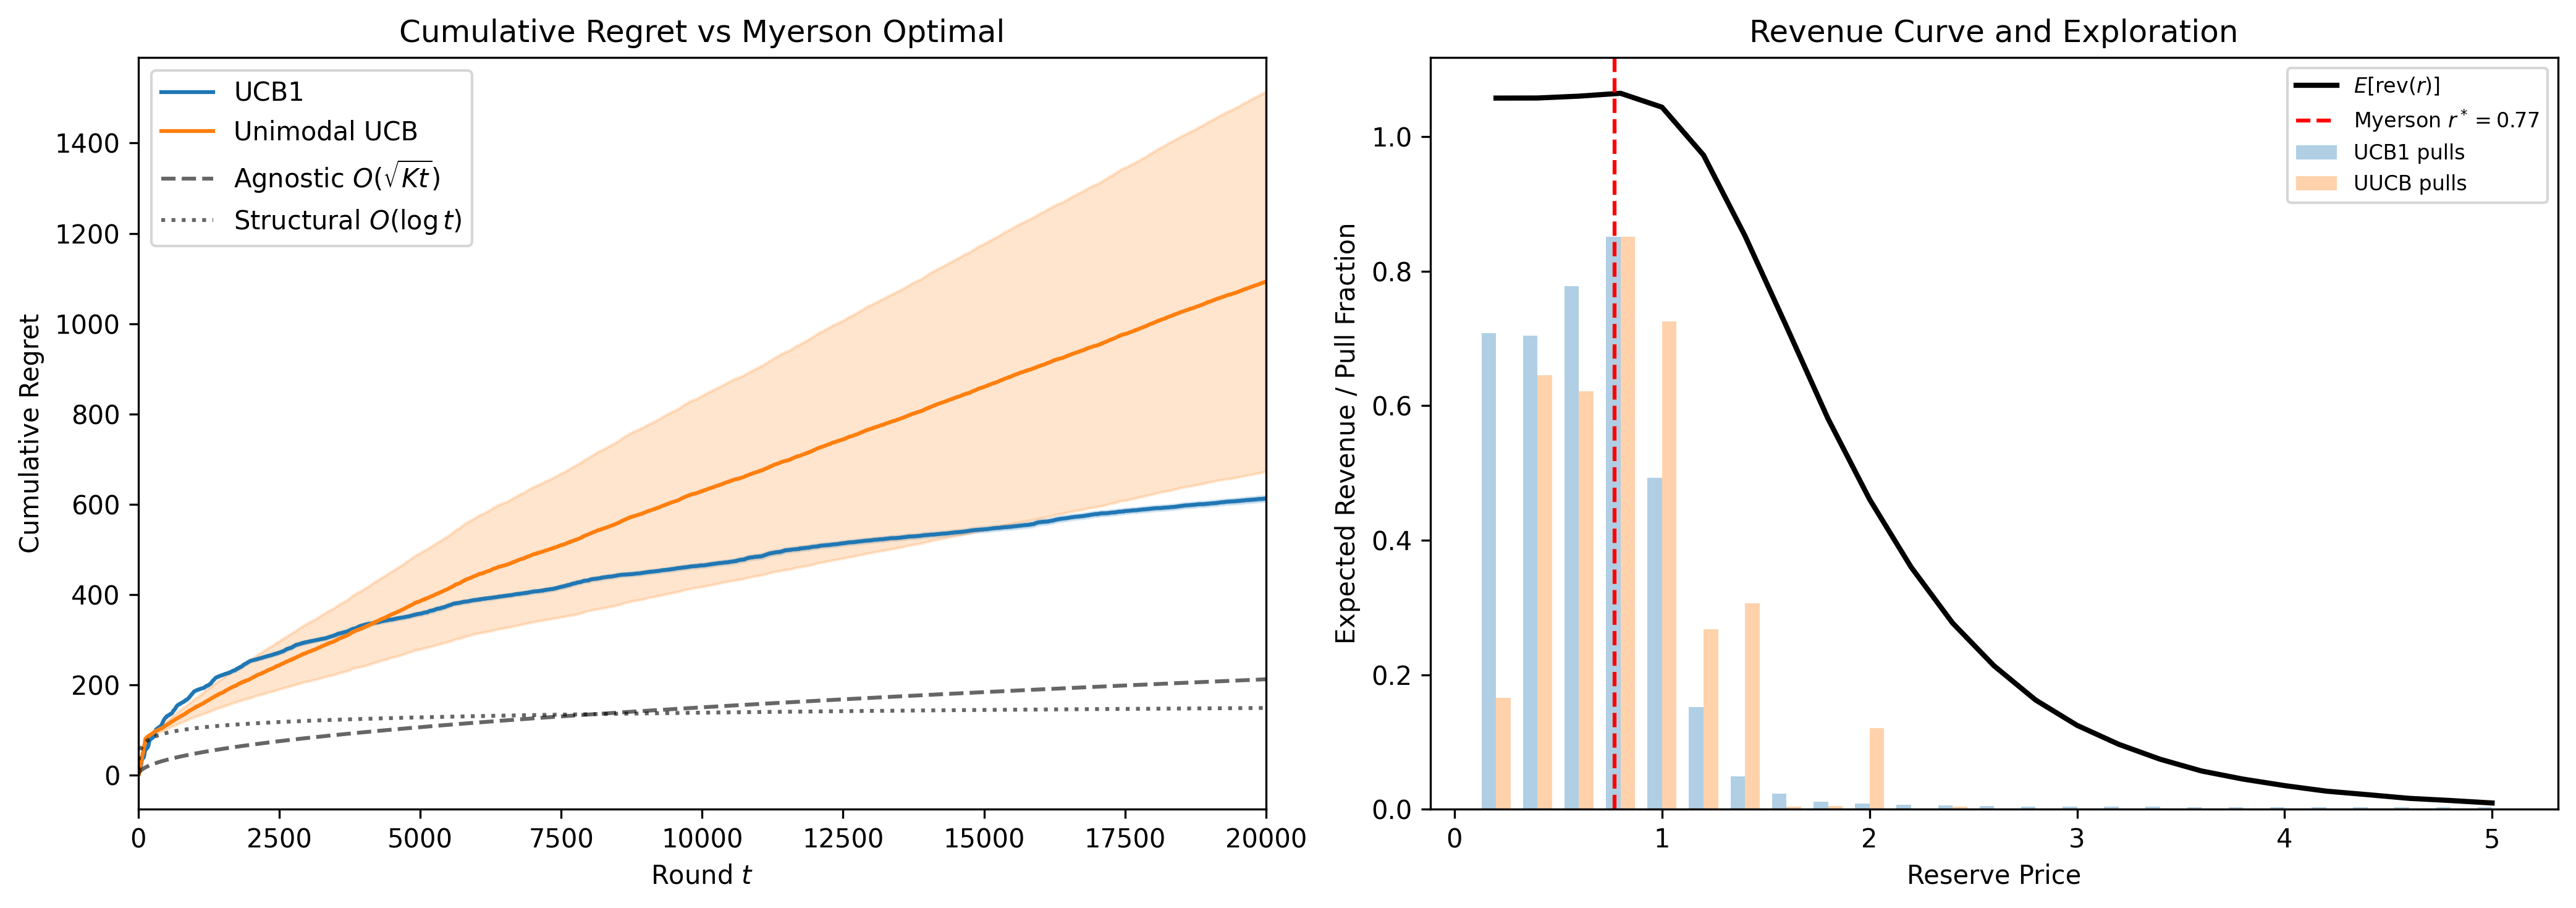
\includegraphics[width=\textwidth]{../ch06_bandits/sims/auction_reserve_regret.png}
\caption{Left: cumulative regret of UCB1 and Unimodal UCB relative to the Myerson oracle for reserve price learning with $N = 3$ LogNormal bidders over $T = 20{,}000$ rounds. Solid lines are means over 30 seeds; shaded regions indicate $\pm 1$ standard error. Right: expected revenue curve over the reserve price grid (black), with overlaid pull distributions for UCB1 (blue bars) and UUCB (orange bars).}
\label{fig:auction_reserve}
\end{figure}

\begin{table}[htbp]
\centering
\begin{tabular}{lcc}
\hline
Algorithm & Final Regret & \% of Myerson Optimum Revenue \\
\hline
UCB1 & $612.8 \pm 5.6$ & $97.12 \pm 0.03\%$ \\
Unimodal UCB & $1093.2 \pm 420.7$ & $94.86 \pm 1.98\%$ \\
Myerson Oracle & $0.0 \pm 0.0$ & $100.00 \pm 0.00\%$ \\
\hline
\end{tabular}

\caption{Terminal cumulative regret and percentage of Myerson optimal revenue for reserve price learning with $N = 3$ LogNormal bidders over $T = 20{,}000$ rounds. Mean $\pm$ one standard error over 30 seeds.}
\label{tab:auction_reserve}
\end{table}


\subsection{Budget-Constrained Bandits}
\label{sec:budget_constraints}

Many economic decisions involve resource constraints. Consider an advertiser bidding in repeated auctions with budget $B$. Let $X_t(a)$ and $C_t(a)$ denote the reward (e.g., clicks) and cost when taking action $a$ at time $t$. The objective is to maximize $\sum_{t=1}^{T} X_t(a_t)$ subject to $\sum_{t=1}^{T} C_t(a_t) \leq B$. \citet{Badanidiyuru2013} frame this as Bandits with Knapsacks (BwK) and introduce a primal-dual approach with dual price $\lambda_t$ for the budget constraint. Given estimates of arm reward $\hat{\mu}_i$ and cost $\hat{c}_i$, the algorithm selects the arm maximizing $\hat{\mu}_i - \lambda_t\hat{c}_i$, capturing the economic principle of marginal value versus marginal cost. This achieves near-optimal $\tilde{O}(\sqrt{T})$ regret while respecting budget constraints.\footnote{The notation $\tilde{O}$ suppresses logarithmic factors, i.e., $\tilde{O}(f(T)) = O(f(T) \cdot \text{polylog}(T))$.}

\citet{Flajolet2017} extend this to contextual bidding for online advertising where click-through and cost distributions depend on observable features $\mathbf{x}_t$. Their UCB-based algorithm combines linear payoff estimation with stochastic binary search, achieving regret $\tilde{O}(d\sqrt{T})$ when the budget scales linearly with $T$.

For combinatorial settings with multiple simultaneous auctions, \citet{Sankararaman2018} exploit economic structure by decoupling auctions but coupling their budgets through a shared Lagrange multiplier. This yields regret that grows polynomially rather than exponentially in the number of auctions, making previously intractable problems computationally feasible.

\citet{Nuara2018} apply similar principles to joint bid and budget optimization across multiple advertising channels. Using Gaussian Process regression to model each subcampaign's click-through function and dynamic programming to enforce budget constraints, they achieved the same conversion volume as human experts with half the cost per acquisition in a two-month field experiment.

\subsubsection{Simulation Study: Budget-Constrained Advertising}
\label{sec:sim_bwk}

We test whether the primal-dual decomposition of \citet{Badanidiyuru2013} enables effective budget management relative to naive and heuristic baselines. The environment has $K = 10$ bid levels on $\{0.50, 1.00, \ldots, 5.00\}$, with competing bids drawn from $\text{Exp}(0.5)$ (mean 2.0) and clicks from $\text{Bernoulli}(0.3)$. The auction is second-price: the advertiser wins if their bid exceeds the competing bid and pays the competing bid as cost. The total budget is $B = 0.3T$ with $T = 10{,}000$.

The LP relaxation benchmark, which solves $\max_{\mathbf{x}} \sum_i x_i \mathbb{E}[X_i]$ subject to $\sum_i x_i \mathbb{E}[C_i] \leq B/T$ and $\sum_i x_i = 1$, yields an optimal reward of $\approx 1{,}461.5$. Three algorithms are compared: (i) UCB1-no-budget, which ignores the budget constraint and selects arms by~\eqref{eq:ucb1}; (ii) proportional pacing, which throttles participation by the fraction of remaining budget $f_t = B_{\text{rem}} / B$, skipping each round with probability $1 - f_t$; and (iii) BwK primal-dual, which maintains a dual variable $\lambda_t$ updated with learning rate $\eta = 1/\sqrt{T}$ and selects the arm maximizing $\hat{\mu}_i - \lambda_t \hat{c}_i + \text{bonus}$. Competing bids and click outcomes are pre-generated for each seed. The experiment is replicated over 30 seeds.

Figure~\ref{fig:bwk} shows three panels: cumulative reward (left), regret relative to the LP relaxation (center), and budget consumption (right). UCB1-no-budget exhausts its budget by approximately round 2{,}000, flatlining at a total reward of $722 \pm 5$. Proportional pacing spreads spending across the horizon but selects arms poorly, achieving only $692 \pm 5$. BwK primal-dual reaches $1{,}292 \pm 6$ (regret $169$ vs the LP benchmark), utilizing the full budget while concentrating on high-reward, low-cost arms as $\lambda_t$ stabilizes. The dual variable rises during early exploration (when expensive arms are sampled) and converges to a level that implicitly selects the LP-optimal mixture. Table~\ref{tab:bwk} reports the full results.

\begin{figure}[htbp]
\centering

\includegraphics[width=\textwidth]{../ch06_bandits/sims/bwk_regret.png}
\caption{Left: cumulative reward for three algorithms under a budget constraint ($B = 0.3T$, $K = 10$ bid levels). Center: cumulative regret relative to the LP relaxation benchmark. Right: budget utilization (cumulative cost as a fraction of $B$). Solid lines are means over 30 seeds; shaded regions indicate $\pm 1$ standard error. The LP benchmark is shown as a dashed black line.}
\label{fig:bwk}
\end{figure}

\begin{table}[htbp]
\centering
\begin{tabular}{lccc}
\hline
Algorithm & Total Reward & Budget Utilization (\%) & Regret vs LP \\
\hline
UCB1-no-budget & $722.2 \pm 4.9$ & $100.0 \pm 0.0$ & $739.3 \pm 4.9$ \\
Proportional Pacing & $691.9 \pm 4.6$ & $96.0 \pm 0.1$ & $769.5 \pm 4.6$ \\
BwK Primal-Dual & $1292.3 \pm 6.4$ & $100.0 \pm 0.0$ & $169.2 \pm 6.4$ \\
\hline
LP Benchmark & $1461.5$ & --- & $0.0$ \\
\hline
\end{tabular}

\caption{Total reward, budget utilization, and regret relative to the LP relaxation for budget-constrained advertising with $K = 10$ bid levels and $B = 0.3T$ over $T = 10{,}000$ rounds. Mean $\pm$ one standard error over 30 seeds.}
\label{tab:bwk}
\end{table}


\subsection{Strategic Interactions}
\label{sec:strategic_interactions}

Economic theory enhances multi-agent reinforcement learning in competitive markets. \citet{Guo2023} study dynamic pricing between firms where consumers follow a logit model with reference price effects:
\begin{equation}
U_t(i) = \alpha_i - \beta p_{i,t} + \gamma(\rho_t - p_{i,t}) + \epsilon_{i,t}
\end{equation}
where $\rho_t$ is the reference price evolving according to:
\begin{equation}
\rho_{t+1} = (1-\delta)\rho_t + \delta\frac{1}{n}\sum_i p_{i,t}
\end{equation}
By incorporating this behavioral economic insight into online projected gradient ascent, they prove $O(1/t)$ convergence to Nash equilibrium, substantially faster than model-free approaches that lack economic structure. The reference price mechanism introduces intertemporal dependence: today's pricing decisions affect future consumer expectations, transforming a static game into a dynamic one. The $O(1/t)$ convergence rate, which matches the optimal rate for strongly convex online optimization, is achieved precisely because the logit demand structure and reference price dynamics together yield a strongly monotone game.

\subsubsection{Simulation Study: Convergence to Nash Equilibrium}
\label{sec:sim_strategic}

We test the Guo (2023) model by comparing a structure-aware gradient method against model-free Q-learning in a symmetric duopoly with reference price effects. The environment has $n = 2$ firms, $T = 5{,}000$ rounds, and consumer utility $U_t(i) = \alpha_i - \beta p_{i,t} + \gamma(\rho_t - p_{i,t}) + \epsilon_{i,t}$ with logit choice (including an outside option normalised to zero). The reference price evolves as $\rho_{t+1} = (1 - \delta)\rho_t + \delta \bar{p}_t$ with $\delta = 0.1$. Parameters are $\alpha_1 = \alpha_2 = 2$, $\beta = 1$, $\gamma = 0.5$. The static Nash equilibrium, computed via iterated best response on a fine grid, is $p^*_{\text{NE}} \approx (1.189, 1.189)$ with per-firm expected profit $0.486$.

Three algorithms are compared: (i) online projected gradient ascent, where each firm updates $p_{i,t+1} = \text{Proj}_{[p_{\min}, p_{\max}]}[p_{i,t} + \eta_t \hat{\nabla}_{p_i} \pi_i]$ using finite-difference gradient estimates and step size $\eta_t = 0.5/(1 + t/50)$; (ii) independent Q-learning, where each firm discretises prices into 20 levels on $[0.1, 5.0]$, maintains a Q-table updated with learning rate $0.1$, and follows a linearly decaying $\varepsilon$-greedy schedule from $\varepsilon = 1.0$ to $0.01$ over $80\%$ of the horizon, with stochastic demand realisations from 100 consumers per round; and (iii) the static Nash oracle, which sets $p^*_{\text{NE}}$ in every round. The experiment is replicated over 30 seeds with random initial prices.

Figure~\ref{fig:strategic_pricing} displays the distance to Nash equilibrium $\|p_t - p^*_{\text{NE}}\|_2$ (left panel) and cumulative industry profit (right panel). Gradient ascent converges to within $0.075$ of the Nash equilibrium, consistent with the $O(1/t)$ rate predicted by the strongly monotone game structure. Its low standard error ($\pm 0.000$) reflects the deterministic dynamics given the expected-profit oracle. Independent Q-learning converges more slowly, stabilising at an average distance of $0.380 \pm 0.036$; the discretisation of the price grid and stochastic demand realisations introduce persistent noise that prevents exact convergence. Both algorithms achieve cumulative profits close to the Nash oracle ($4{,}864$): gradient ascent reaches $4{,}701 \pm 1$ and Q-learning $4{,}711 \pm 45$. The profit gap between the learning algorithms and the oracle reflects exploration costs during the initial transient phase. Table~\ref{tab:strategic_pricing} reports the full results.

\begin{figure}[htbp]
\centering
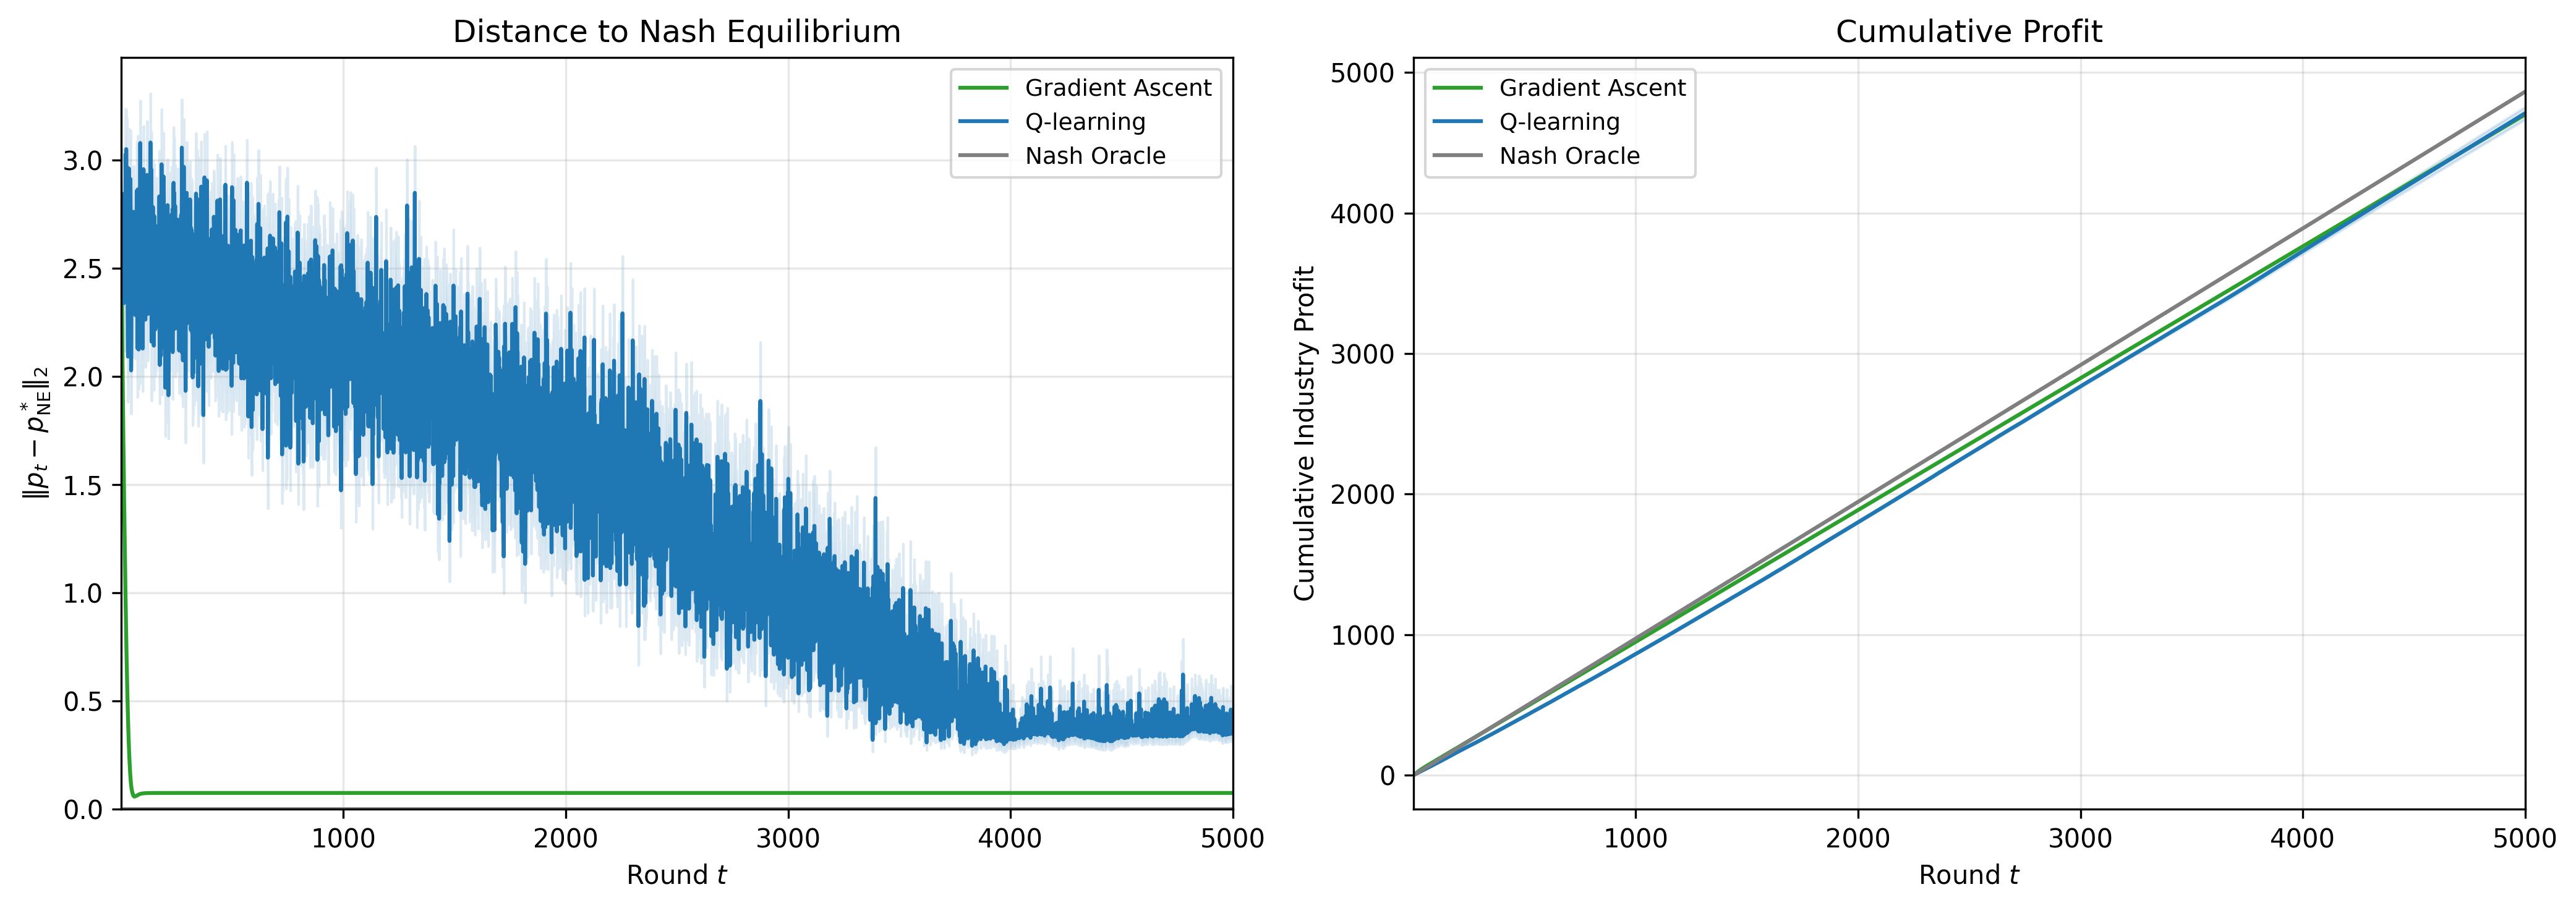
\includegraphics[width=\textwidth]{../ch06_bandits/sims/strategic_pricing_convergence.png}
\caption{Left: distance to Nash equilibrium $\|p_t - p^*_{\mathrm{NE}}\|_2$ for two-firm logit pricing with reference effects ($\gamma = 0.5$, $\delta = 0.1$) over $T = 5{,}000$ rounds. Right: cumulative industry profit (sum over both firms). Solid lines are means over 30 seeds; shaded regions indicate $\pm 1$ standard error.}
\label{fig:strategic_pricing}
\end{figure}

\begin{table}[htbp]
\centering
\begin{tabular}{lcc}
\hline
Algorithm & Avg.\ Distance to NE (last 500) & Cumulative Industry Profit \\
\hline
Gradient Ascent & $0.0752 \pm 0.0000$ & $4701.2 \pm 1.2$ \\
Q-learning & $0.3799 \pm 0.0355$ & $4710.9 \pm 45.3$ \\
Nash Oracle & $0.0000 \pm 0.0000$ & $4863.8 \pm 0.0$ \\
\hline
\end{tabular}

\caption{Average distance to Nash equilibrium over the last 500 rounds and cumulative industry profit for the two-firm strategic pricing game over $T = 5{,}000$ rounds. Mean $\pm$ one standard error over 30 seeds.}
\label{tab:strategic_pricing}
\end{table}


\subsection{Discussion}
\label{sec:bandits_discussion}

Economic structure improves bandit regret from the agnostic $O(\sqrt{T})$ minimax rate to $O(\log T)$ or $O(\text{poly}(\log T))$ when demand regularity conditions hold, reduces dimensionality from product count $N$ to intrinsic dimension $d$, and preserves near-optimal rates under budget constraints via primal-dual decomposition. The tradeoff is robustness: when structural assumptions fail, misspecification can produce linear regret, so practitioners should prefer structural methods when the economic model is well-supported but monitor for persistent underperformance relative to an agnostic baseline.
